\section{Schaltungen}
\subsection{Zweipole}
\begin{center}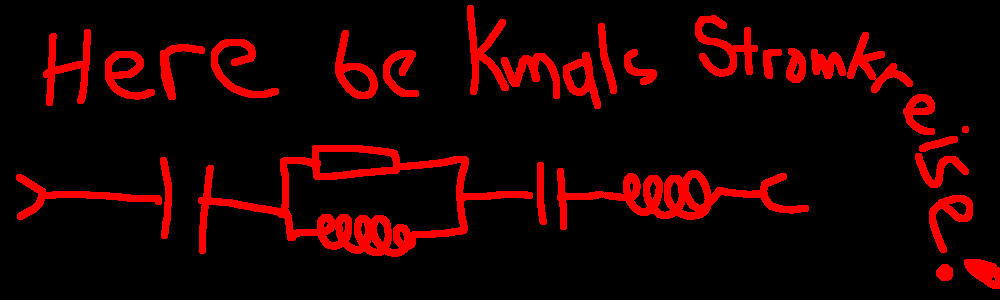
\includegraphics[width=.6\textwidth]{placeholder.png}\end{center}~\\
%
% Ne Figure mit 4 Subfigures, wenn du dass hinbekommst.
% Ne RC Reihe, Ne RC Parallel, Ne RL Reihe, Ne RL Parallel, ne RLC Reihe. (Z_1 - Z_5)
%
Für jede dieser Schaltungen lässt sich recht einfach die Gesamtimpedanz berechnen, aus der wir dann
die anderen Größen erhalten, welche wir schließlich Interpretieren wollen.
Es sei $R=\SI{1}{\kilo\ohm},\, C=\SI{1}{\nano\farad},\, L=\SI{1}{\henry}$ und $\omega = 1,10^3,10^{9} \si{Hz}$.
% normale werte, eisenkernspule
In dem selben Stil lassen sich auch die Impedanzen von komplexeren Kombinationen
von Reihen- und Parallelschaltungen berechnen. Auch die Lösung des linearen Gleichungssystems aus den Kirchhoffschen Gesetzen für noch kompliziertere Schaltungen geht analog zur Behandlung von Schaltungen aus Widerständen.
\begin{align*}
    && &\qquad \omega = \SI{1}{\Hz} &&\qquad \omega = \SI{1e3}{\Hz} &&\qquad \omega = \SI{1e9}{\Hz} \\
    Z_1 &= R + \ic 
    &&= (10^3 - 10^9 \imu)\,\si{\ohm} &&=(10^3 - 10^6 \imu)\,\si{\ohm} &&=(10^3 - \imu)\,\si{\ohm} \\
    Z_2 &= R \parallel \ic = \frac{1}{\frac{1}{R} + \imu \omega C}
    &&\approx (10^3 - 10^{-3} \imu)\,\si{\ohm} &&\approx(10^3 - \imu)\,\si{\ohm} &&\approx(10^{-3} - \imu)\,\si{\ohm} \\
    Z_3 &= R + \il 
    &&= (10^3 - \imu)\,\si{\ohm} &&=(10^3 - 10^3 \imu)\,\si{\ohm} &&=(10^3 - \imu)\,\si{\ohm} \\
    Z_4 &= R \parallel \il = \frac{1}{\frac{1}{R} + \frac{1}{\il}} 
    &&\approx (10^{-3} - \imu)\,\si{\ohm} &&\approx(500 - 500 \imu)\,\si{\ohm} &&\approx(10^3 - 10^{-3}\imu)\,\si{\ohm} \\
    Z_5 &= R + \il + \ic 
    &&= (10^3 - 10^9\imu)\,\si{\ohm} &&\approx(10^3 - 10^6 \imu)\,\si{\ohm} &&=(10^3 + 10^9\imu)\,\si{\ohm} 
\end{align*}
% wär irgendwie cool, wenn wir |Z_n| über w plotten könnten. Bock das zu machen?
Man sieht das typische Verhalten der passiven Bauteile. Der Scheinwiderstand einer Spule verringert 
sich für geringere Frequenzen, der eines Kondensators für hohe Frequenzen.
Für RC/RL Reihenschaltungen führt dies zu einer Frequenzabhängigen Phasendifferenz $\arctan(\tfrac{X_{C/L}}{R})$, der Scheinwiderstand fällt/wächst mit steigender Frequenz, bleibt aber strikt größer als $R$.
Für die RC/RL Parallelschaltungen verhält es sich entgegengesetzt analog.
Bemerkenswert ist dabei, dass dadurch der Wirkwiderstand reduziert werden kann.
$Z_5$ stellt die Gesamtreihenschaltung aus $R$, $C$ und $L$ dar, und besitzt einen minimalen Scheinwiderstand von $R$ und Blindwiderstand von $0$ bei einer Grenzfrequenz $f_g = 10^{4.5}\si{\hertz}$, bei der sich die beiden Blindwiderstandsanteile genau aufheben.
Legt man z.B. die Amplitude der Spannung über die beiden Pole fest, so kann man mit diesen Schaltungen Strom so steuern, dass er nur bei hohen Frequenzen, niedrigen Frequenzen, mittleren Frequenzen oder alles außer mittleren Frequenzen fließt. Betrachtet man den Spannungsanteil, der bei verschiedenen Frequenzen über ein Teilbauteil abfällt und nimmt diesen als Output, so kann man damit auch Spannungen über die Frequenz regeln. Man siehe Kapitel (?).
%%% ICH HAB VERGESSEN WIE LABELS WORKEN UND BIN FAUL

Überlegt man sich jedoch, wie sich die LC-Kreise wie $Z_5$ ohne Widerstand speziell bei $f_g$ verhalten, dann kommt man zu Schwingkreisen.

\begin{center}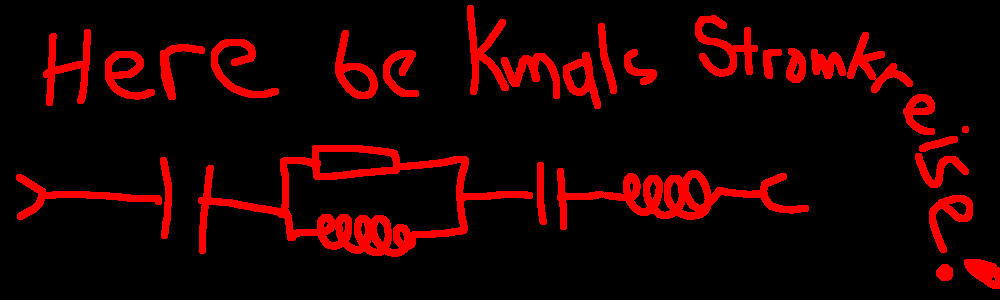
\includegraphics[width=.6\textwidth]{placeholder.png}\end{center}~\\
%
% Ne Figure mit 4 Subfigures, wenn du dass hinbekommst.
% die selbe RLC Reihe, Ne LC Reihe, Ne RLC Parallel, Ne RLC Parallel. (Z_5 - Z_8)
%
\begin{align*}
    \qquad&&Z_5 &= R + \il + \ic & \xrightarrow{R \,\rightarrow \,\SI{0}{\ohm}} && \il + \ic &= Z_6 
    &&\qquad\\
    \qquad&&Z_7 &= R \parallel \il \parallel \ic & \xrightarrow{R \,\rightarrow \,\SI{0}{\ohm}} && \il \parallel \ic &= Z_8 &&\qquad\\
\end{align*}
In Schaltung $Z_5$ und $Z_6$ verringert sich der Blindwiderstand nach der Wechselstromrechnung bei höheren Frequenzen auf 0 und steigt dann bei noch höheren Frequenzen wieder vom Betrag her an.
Warum? Weil sie bei dieser Frequenz einen (un)gedämpften Schwingkreis darstellt, welcher mit Resonanzfrequenz betrieben wird, weswegen die Schaltung keine Arbeit verrichtet, da Sie sich von selber in Schwingung befindet.
Schaltungen $Z_7$ und $Z_8$ beschreiben den selben Schwingkreis, an welchen nun allerdings von außen 
Spannung angelegt wird. diese Spannung erzeugt bei im Ungedämpften Kreis bei der Resonanzfrequenz jedoch nur einen Fluss innerhalb der Schaltung, da der Kondensator genau den Strom nimmt, den die Spule gibt.
% DIE DUDS KÖNNEN SCHWINGKREISE; DESWEGEN ERKLÄR ICH DAS HIER NICH LANG UND BREIT
Die Wechselstromrechenmethode ist hier also in der Lage, die Effekte solcher Schwingungen richtig vorherzusagen.
\begin{align*}
    Z_6 &\stackrel{!}{=} 0 &\implies&& \il &= -\ic &\implies&& \omega^2 &= \frac{1}{LC} \eqqcolon f_{g}^2\\
    Z_8 &\stackrel{!}{=} \infty &\implies&& \frac{1}{\imu \omega L} &= -\imu \omega C &\implies&& \omega^2 &= \frac{1}{LC} = f_{g}^2\\
\end{align*}